\section{L'architecture} \label{sec:micro}
%%%%%%%%%%%%%%%%%%%%%%%%%%%%%%%%%%%%%%%%%%%%%%%%%%%%%%%%%%%%%%%%%%%
%%%%%%%%%%%%%%%%%%%%%%%%%%%%%%%%%%%%%%%%%%%%%%%%%%%%%%%%%%%%%%%%%%%

Dans la section \autoref{sec:logique} sont présentés les transistors, les éléments de bases des ordinateurs. Les transistors sont groupés en portes logiques pour construire des circuits électroniques. Cette section présente comment ces circuits sont utilisés pour construire la microarchitecture d'un ordinateur capable d'exécuter les instructions définies par une \textit{Instruction Set Architecture} (ISA). L'objectif n'est pas de présenter la totalité de l'architecture, mais seulement les éléments importants nécessaires pour la suite de la thèse.

Afin d'éviter toutes confusions, nous rappelons la définition de la microarchitecture et de l'ISA car ces termes sont souvent confondus dans la littérature:

\begin{itemize}
    \item  \textbf{La couche ISA} (\textit{Instruction Set Architecture}) regroupe les instructions, leur mode (système ou utilisateur), les registres utilisables, l'organisation du système mémoire (alignement, espace d'adressage) ... 
    C'est une spécification formelle établie, qui peut être utilisée par plusieurs fabricants de microarchitectures \cite{tanenbaum2016structured}. Intel publie fréquemment la documentation de l'ISA x86 \cite{guide2011intel}. Elle forme l'interface entre le matériel et le logiciel et permet la compatibilité de programme sur des microarchitectures de différents constructeurs. 
    Grâce à la couche ISA, différents langages de programmation peuvent être utilisés pour écrire les applications. Le compilateur s'occupe alors de les traduire dans un langage de bas niveau pouvant utiliser l'ISA (langage assembleur). Ce langage est tellement proche de la couche ISA que les deux termes sont souvent mélangés. Les \textit{ISA} existantes sont listées dans la \autoref{sec:isa}. 

    \item \textbf{La microarchitecture} correspond à l'implémentation matérielle de l'\textit{ISA}. Ce sont deux couches distinctes, la seconde n'ayant pas forcément besoin d'avoir connaissance de la première (bien que pour des raisons de performances cela soit préférable). En ayant connaissance de la microarchitecture, le compilateur pourra réordonner ou modifier des instructions pour tirer parti du pipeline ou d'un processeur vectoriel. La conception d'une nouvelle microarchitecture doit commencer par choisir l'ISA à implémenter (si possible existante pour permettre la compatibilité des programmes). Les différences principales entre deux microarchitectures implémentant la même ISA sont leur différence de performances et de coût. Les processeurs Intel et AMD implémentent la même \textit{ISA x86}. La performance et le nombre d'instructions supportés par les deux architectures sont cependant différents.
    
    \item Le terme d'\textbf{architecture} est souvent employé à la place du terme \textit{ISA}, notamment par IBM en 1964 \cite{amdahl1964architecture}.  Aujourd'hui il est souvent utilisé pour faire référence à la fois à l'\textit{ISA} et à la \textit{microarchitecture}. Il est courant d'entendre parler d'\textit{architecture x86} pour faire référence à une microarchitecture implémentant l'\textit{ISA x86}.\\ 
\end{itemize}



\subsection{Performance d'une architecture}
%%%%%%%%%%%%%%%%%%%%%%%%%%%%%%%%%%%%%%%%%%%%%%%%%%%%%%%%%%%%%%%%%%%


Le développement d'une nouvelle microarchitecture doit prendre en compte plusieurs facteurs qui peuvent impacter son implémentation (vitesse de traitement des instructions, le coût de fabrication, la fiabilité, consommation électrique, taille). Ces différents facteurs font pression sur les architectes de processeurs qui doivent redoubler d'inventivité pour les satisfaire en implémentant des optimisations matérielles.

Les améliorations ont pour but d'améliorer la performance de l'architecture, la plupart du temps de façon transparente pour l'utilisateur. Cependant, un programmeur n'étant pas averti de ces optimisations, pourraient écrire des applications inefficaces, voire contre-productives. Les développeurs d'applications \textit{HPC} étant généralement des scientifiques experts dans leur domaine (physique, chimie, mécanique…), il est fréquent de voir des codes peu efficaces. Cette section liste les principales améliorations des microarchitectures qu'il faut connaître et utiliser pour exploiter le maximum des performances disponibles. 


Pour améliorer la vitesses d'exécution d'un programme, quatre moyens peuvent être utilisés:
\begin{itemize}
    \item Utiliser une nouvelle technologie, plus rapide, consommant moins d'énergie, moins chère ou plus dense (\autoref{sec:opportunité}). 
    \item Améliorer l'efficacité des instructions (\autoref{sec:efficacite}) 
    \item Accélérer l'exécution des instructions: (\autoref{sec:accelerer})
    \item Exécuter les instructions en parallèle: (\autoref{sec:para})
\end{itemize}

Quand elles ne sont pas matérielles, ces différentes améliorations peuvent être réalisées par deux techniques: dynamique ou statique. Les méthodes statiques interviennent avant que le code soit exécuté. Généralement, c'est le compilateur qui les implémente lors de la génération du code. Les techniques dynamiques sont mis en oeuvre au fil des exécutions d'instructions. Elles nécessitent donc du matériel spécialisé supplémentaire et sont donc très coûteuses. La section présente les principales techniques et matériels utilisés pour l'amélioration des performances (dynamique et statique). Deux améliorations majeures sont présentées dans deux sections distinctes: la hiérarchie mémoire (\autoref{sec:hierarchie}) et la mémoire virtuelle (\autoref{sec:memoire_virtuelle}).







%%%%%%%%%%%%%%%%%%%%%%%%%%%%%%%%%%%%%%%%%%%%%%%%%%%%%%%%%%%%%%%%%%%
\subsection{Améliorer l'efficacité de l'exécution} \label{sec:efficacite}
%%%%%%%%%%%%%%%%%%%%%%%%%%%%%%%%%%%%%%%%%%%%%%%%%%%%%%%%%%%%%%%%%%%




\subsubsection{Jeu d'instructions ISA } \label{sec:isa}
%%%%%%%%%%%%%%%%%%%%%%%%%%%%%%%%%%%%%%%%%%%%%%%%%%%%%%%%%%%%%%%%%%%

Le choix de l'\textit{ISA} à implémenter est le premier choix à réaliser lors du développement d'une nouvelle microarchitecture. L'\textit{ISA} utilisé à un impact sur la performance, la facilité de programmation et sur la compatibilité des applications existantes. Les jeux d'instructions couramment utilisés sont séparés en deux grandes familles d'ISA: les jeux d'instructions CICS pour \textit{Complex Instruction Set Computing} et les instructions RISC pour \textit{Reduced Instruction Set Computing}. La principale différence entre les deux est la complexité de leurs instructions. 

    \paragraph{CISC} est la première famille d'instructions à avoir été utilisée massivement. Ces instructions sont dites complexes, car une seule instruction peut à elle seule demander plusieurs opérations à réaliser. Par exemple, une addition CISC s'occuperait de charger les données depuis la mémoire, d'exécuter l'addition pour ensuite sauver le résultat. À l'origine, beaucoup de codes étaient écrits en assembleur, et ce genre d'instructions permettaient au programmeur d'éviter d'écrire de nombreuses lignes de codes souvent redondantes. De plus, les codes générés en CISC sont plus petits et nécessitent donc moins de mémoire, qui à l'origine manquait énormément.

    \paragraph{RISC} regroupe les ISA dites \textit{simple}. En 1970, John Cocke, alors ingénieur chez IBM, proposa de réduire le nombre d'instructions CISC \cite{cocke1990evolution}. Le terme \textit{réduit} fait référence au nombre d'instructions plus petit que celles de CISC, mais aussi pour signifier que le travail à réaliser par une instruction était moindre que pour une instruction CISC. Pour réaliser une multiplication entre deux données, on devra alors explicitement charger la première donnée, puis la deuxième et enfin écrire l'instruction qui correspond à la multiplication. Les instructions étant plus nombreuses, le travail des compilateurs est augmenté, mais souvent l'exécution des codes résultante en est réduite. Le RISC fut une réponse apportée à la lenteur de décodage du CISC.  Toutes les instructions font la même taille, les architectures nécessitent donc moins de transistors pour les analyser. Les microarchitectures sont donc moins coûteuses et peuvent atteindre des fréquences plus élevées.


Ces deux familles d'instructions ont toutes deux leurs avantages et leurs inconvénients et les puces actuelles comportent des parties qui exécutent des instructions RISC et d'autres en CISC. L'ISA la plus répandue est le x86 qui se veut être un jeu d'instruction CISC. Le RISC augmente le nombre d'instructions lues séparément par le microprocesseur, si cela a le désavantage de consommer plus de mémoire, cela a aussi d'autres avantages, comme de pouvoir optimiser leur exécution avec la mise en place d'un \textit{pipeline}. Les ISA RISC les plus connus sont les ISA ARM, MIPS (utilisé dans le domaine universitaire pour apprendre le langage assembleur), PA-RISC (Hewlett-Packard) et RISC-V. L'ISA CISC la plus utilisée dans les supercalculateurs aujourd'hui est \textit{x86} (processeurs Intel et AMD).



\paragraph{Extensions vectorielles.}
Pour tirer partie de la puissance de calculs des processeurs et des unités de calculs vectorielles, les \textit{ISA} ont reçu de nombreuses extensions (\autoref{tab_simd}).
C'est en 1995 que Sun Microsystem introduit son premier jeu d'instruction vectoriel, le Visual Instruction Set auquel Intel répondra en 1997 avec son processeur Pentium MMX et le jeu d'instructions du même nom. Ainsi ces instructions pouvaient réaliser des opérations sur les jeux de données tels que les images ou vidéos de façon très performante. En 1997 AMD viendra améliorer le jeu d'instruction MMX avec l'implémentions des instructions 3DNow ! qui rendait alors possible les opérations vectorielles sur les nombres flottants. La possibilité de faire une opération sur deux nombres flottant par cycle doublait alors la performance des processeurs. Intel répondit alors à cette avance avec le jeu d'instructions Streaming SIMD Extensions (SSE) en 1999. Il est alors facile d'augmenter la puissance des processeurs : il suffit d'augmenter la taille des vecteurs.
L'\textit{ISA x86} a reçu plus de dix extensions dans les vingt dernières années pour s'adapter l'agrandissement des unités vectorielles. Les principales sont \textit{MMX} (1996), \textit{3DNOW!} (1998), 6 versions de \textit{SSE} de 1999 2008 et enfin \textit{AVX-2} et \textit{AVX-512} en 2013 et 2015. Évidemment, les codes ne peuvent pas profiter de ces instructions sans une microarchitecture capable de les exécuter. Ces microarchitectures sont présentes dans la sous-section suivante. 


\begin{table}[]
\centering
\caption{Évolutions principales des instructions SIMD $x86$}
\label{tab_simd}
\begin{tabular}{|l|l|l|l|l|l|}
\hline
\multicolumn{1}{|c|}{\textbf{Année}} & \multicolumn{1}{c|}{\textbf{Nom}} & \multicolumn{1}{c|}{\textbf{Nb registres}} & \multicolumn{1}{c|}{\textbf{Taille (bit)}} & \multicolumn{1}{c|}{\textbf{Registres}} & \multicolumn{1}{c|}{\textbf{Commentaires}} \\ \hline
1996                                 & MMX                               & 8                                          & 64                                         & MM0                                     & Nombre entiers
\\ \hline
1999                                 & SSE                               & 8                                          & 128                                        & XMM0                                    & 120 instr., simple precisions              \\ \hline
2006                                 & SSSE3                             & 8                                          & 128                                        & XMM0                                    & 300 instr., double précisions              \\ \hline
2008                                 & AVX                               & 16                                         & 128                                        & XMM0                                    & FMA4, op. a 3 opérandes                    \\ \hline
2011                                 & AVX2                              &  16                                          & 256                                        & YMM0                                    &                                            \\ \hline
2013                                 & AVX512                            & 32                                         & 512                                        & ZMM                                     & FMA3                                       \\ \hline
\end{tabular}
\end{table}

\begin{figure}
    \center
    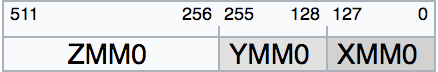
\includegraphics[width=7cm]{images/Chapitre1/simd_registres.png}
    \caption{\label{pic_simd_registres} Découpage d'un registre de 512 bits}
\end{figure}

\subsubsection{Les processeurs vectoriels } \label{sec:cpu_vectoriel}
%%%%%%%%%%%%%%%%%%%%%%%%%%%%%%%%%%%%%%%%%%%%%%%%%%%%%%%%%%%%%%%%%%%

Dans les années 90, les ordinateurs personnels commençaient à être utilisés pour le multimédia (film, image, musique). Dans le but d'augmenter la performance des applications, les architectes ont voulu améliorer l'efficacité des instructions en implémentant des architectures SIMD (Single Instruction Multiple Data de la taxonomie de Flynn ). 

L'architecture vectorielle repose sur les mêmes fondements que l'architecture superscalaire (voir \autoref{sec:superscalar}): réduire le temps d'exécution d'un code en utilisant le parallélisme et diminuer le coût en transistors de la microarchitecture par la mise en commun du matériel entre plusieurs unités de calculs (\autoref{pic_cpu_simd}). La pression que subit l'unité responsable du \textit{fetch} et du \textit{decode} est donc réduite, car avec une seule instruction vectorielle, le processeur réalise le travaille de plusieurs instructions scalaires.  Contrairement au processeur scalaire qui exécute une instruction sur une seule donnée, les processeurs vectoriels sont capables d'exécuter une instruction sur plusieurs données simultanément (\autoref{pic_simd2}).


Ainsi, doubler la largeur des instructions revient à doubler le nombre de FLOP réalisables par le processeur alors que la consommation électrique augmentera d'un facteur inférieur à 2. Beaucoup d'efforts ont donc été réalisés pour être capables d'utiliser cette technologie. Par exemple la majorité des compilateurs est capable de détecter les zones de codes parallélisable pouvant bénéficier d'instructions SIMD.

Cependant, dans la pratique les codes ne sont pas aussi parallèles que nous le souhaiterions et certains aspects du code empêchent de tirer la totalité de la performance disponible. En effet, si les données sont indépendantes les unes des autres, il est alors impossible de les calculer simultanément rendant la partie vectorielle inutilisable. Aussi, les performances peuvent être réduites si les données accédées ne sont pas continues en mémoire. Cela demande donc un travail supplémentaire pour repenser les structures de données et s'assurer que les donnes transférées sur le bus mémoire sont des données utiles (voir le concept de ligne de cache dans la \autoref{sec:cache}).

\begin{figure}
    \begin{subfigure}[]{0.5\linewidth}\centering
        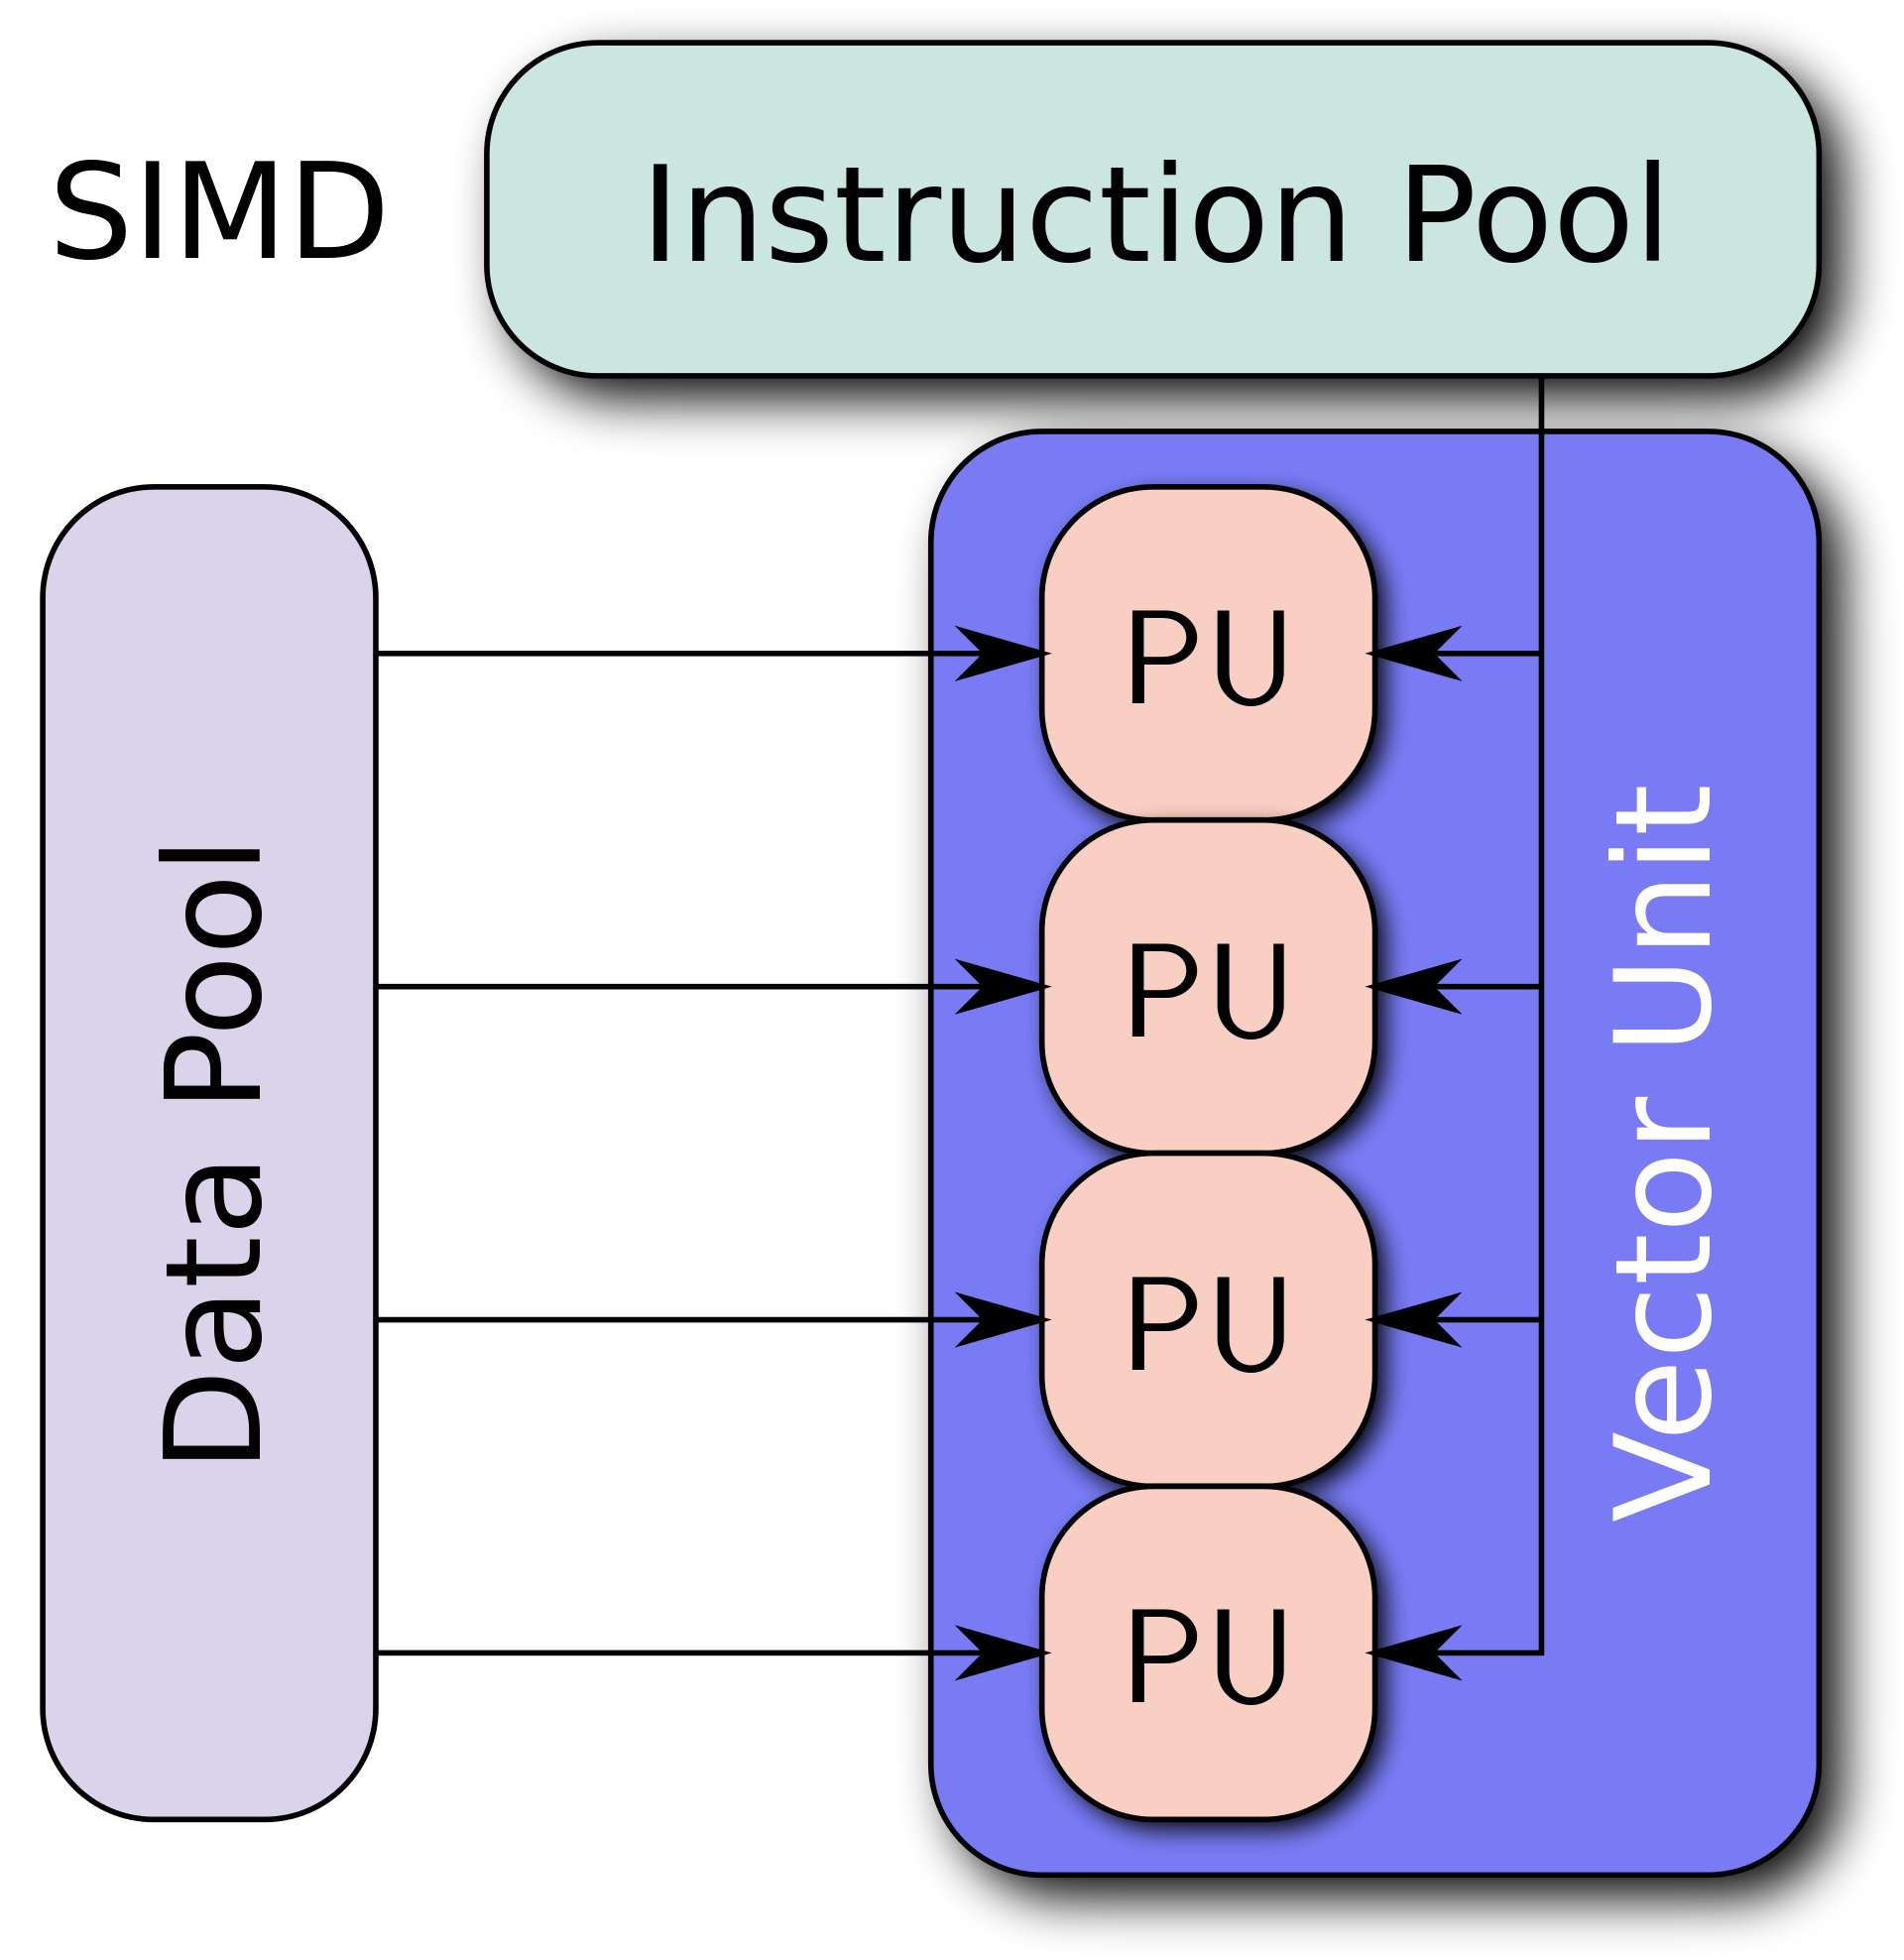
\includegraphics[width=.5\linewidth]{images/cpu_simd.png}
        \caption{Un processeur vectoriel exécute une même instruction sur différentes données
        \label{pic_cpu_simd}}
    \end{subfigure}%
    ~ %space
    \vspace{2.0cm}
    \begin{subfigure}[]{0.8\linewidth}\centering
        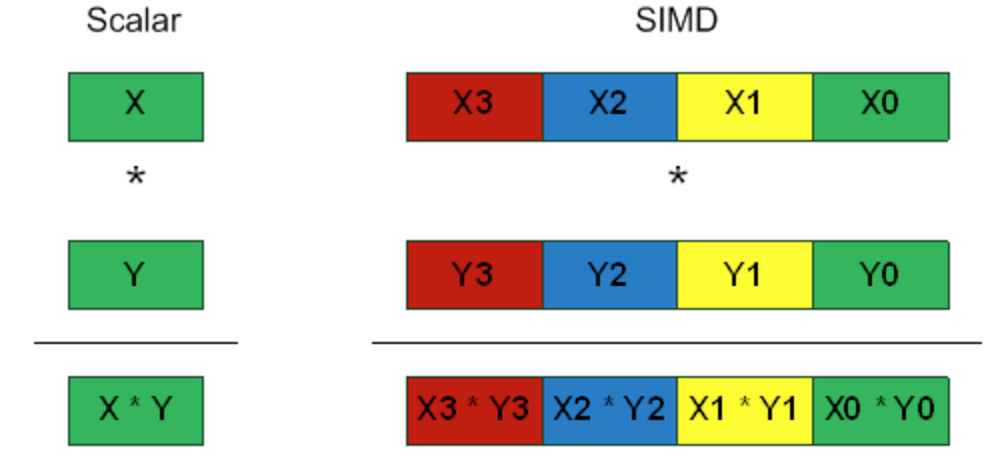
\includegraphics[width=\linewidth]{images/Chapitre1/simd.png}
        \caption{Schéma de fonctionnement d'une multiplication vectorielle\protect\footnotemark}
        \label{pic_simd2}
    \end{subfigure}
   
    \caption{Un processeur vectoriel travaille sur un groupe de données indépendantes. Les opérandes sont alors stockées dans des registres vectoriels capable de charger un vecteur pour y appliquer une même opération.}
    \label{pic_simd}
\end{figure}
\footnotetext{source:\url{https://software.intel.com/en-us/articles/ticker-tape-part-2}}


%%%%%%%%%%%%%%%%%%%%%%%%%%%%%%%%%%%%%%%%%%%%%%%%%%%%%%%%%%%%%%%%%%%
\subsection{Accélérer l'exécution des instructions} \label{sec:accelerer}
%%%%%%%%%%%%%%%%%%%%%%%%%%%%%%%%%%%%%%%%%%%%%%%%%%%%%%%%%%%%%%%%%%%

Utiliser des instructions plus efficaces telles que les instructions vectorielles ou les FMA est un premier moyen d’améliorer la puissance de calcul d’un processeur. Un deuxième moyen est de les exécuter plus rapidement. Cela peut être réalisé en accélérant la fréquence d’un processeur, ou en utilisant des matériels spécialisés pour l’exécution de ces instructions.

\subsubsection{Lien entre fréquence et performance} \label{sec:frequency}
Les processeurs sont des circuits électroniques dits \textit{synchrones}. Leur fonctionnement est cadencé par une horloge donnant des impulsions régulières aux composants du circuit pour organiser leur synchronisation. Lorsqu'une instruction est exécutée par le processeur les passages dans les différentes étapes de la microarchitecture et notamment du pipeline (voir \autoref{sec:pipeline}) sont régis par cette horloge. Au plus l'horloge est rapide, au plus l'exécution du programme l'est aussi. Cependant, la durée séparant deux signaux (un cycle) ne peut pas être réduite à l'infini. En effet, les vitesses d'horloges sont si rapides, qu'il est nécessaire de laisser suffisamment de temps au signal électrique de se propager dans le circuit. La taille du processeur et sa fréquence sont donc liées, c'est notamment pour cette raison qu'il n'existe pas de processeur mesurant plusieurs dizaines de centimètres. À une fréquence de 3 GHz, le signal électrique, qui se déplace à la vitesse de la lumière, ne peut parcourir que quinze centimètres entre deux cycles. En plus du temps de propagation, il faut aussi prévoir le temps de préparer et recevoir la communication. L'augmentation de la fréquence des processeurs a donc une première limite physique infranchissable bien que d'autres limites présentées dans cette partie soient encore plus contraignantes.

La fréquence des processeurs a beaucoup évolué depuis les premiers processeurs (\autoref{pic_cpu_frequency}). Les premiers processeurs \textit{Pentium} d'Intel utilisaient des fréquences de 60 MHz en 1993. Pendant plus de dix ans, les fréquences ont évolué chaque année d'un facteur de 40\%  tous les ans pour atteindre des vitesses de plusieurs Gigahertz. En 2000, Intel annonçait la fabrication de processeurs cadencés à 10 GHz\footnote{source \url{https://www.clubic.com/actualite-1791-des-processeurs-intel-10-ghz-pour-2005.html}} pour les années 2005. Pourtant, en 2019, nous sommes encore loin d’utiliser des processeurs avec de telles cadences. Mis à part les systèmes surcadencés, utilisant des systèmes de refroidissement liquide, il est rare de voir des systèmes utiliser des processeurs récents à plus de 5 GHz.
.
\begin{figure}
    \center
    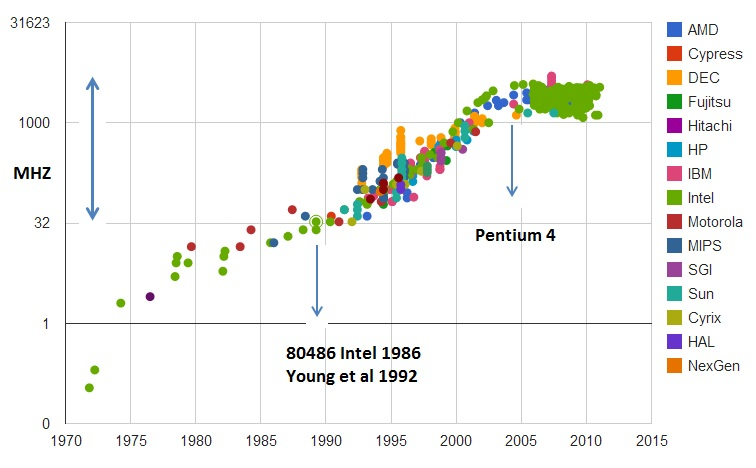
\includegraphics[width=10cm]{images/cpu_frequency.jpg}
    \caption{\label{pic_cpu_frequency} Évolution de la fréquence des processeurs\protect\footnotemark.}
\end{figure}
\footnotetext{source: \url{https://en.wikipedia.org/wiki/Beyond_CMOS}}

Le but de cette section est de comprendre pourquoi l'évolution de la fréquence des processeurs s'est arrêtée brusquement autour des 4 GHz. Pour cela, nous expliquons comment la loi de Moore a permis d'en arriver là, et quelles sont les limites physiques qui empêchent de poursuivre cette évolution.


\subsubsection{Loi de Dennard}\label{sec:denard}
Comme constaté dans la section précédente, la fréquence de l'horloge d'un processeur est limitée par le temps nécessaire au signal de se propager entre deux éléments d'un circuit. Plus les transistors seront proches, plus la vitesse de propagation sera faible. La loi de Moore prévoit que le nombre de transistors double tout les deux ans pour une surface donnée. Cela est rendu possible par l'affinement de la gravure permettant de réaliser des transistors toujours plus petits et donc plus proches. Avec plus de transistors, les processeurs peuvent utiliser des pipelines plus complexes, entre divisant les étapes les plus longues permettant aussi l'utilisation de fréquence plus élevée. Nous expliquons comment l'évolution de la fréquence des processeurs est intimement liée avec la loi de Moore en utilisant la formule de la consommation électrique d'un circuit CMOS \cite{martin2014post}:
\begin{equation}
P = QfCV^{2} +  VI_{leakage}
\label{eq:power}
\end{equation}


L'intérêt de cette formule est d'apprécier comment la puissance et la fréquence d'un processeur est impactée par la loi de Moore. Pour cela, nous étudions sa variation entre deux générations de processeurs, c'est-à-dire une période de deux ans.


\paragraph{Le nombre de transistors $Q$.} D'après la loi de Moore, le nombre de transistors double tous les deux ans pour deux circuits de mêmes surfaces. Ainsi la surface des transistors est divisée par deux. Leur longueur et  leur largeur est ainsi réduite d'un facteur $\sqrt{2}$. Cette valeur est appelée facteur de \textit{scaling} et a une valeur de $1.44$.

\paragraph{La capacité du circuit $C$.} La capacité d'un transistor peut être calculée par la formule suivante $C = \frac{S \times e}{d}$. Avec $S$ la surface du transistor, $e$ la permittivité électrique du matériau utilisé (pouvant être considéré comme fixe entre deux générations), et $d$ la distance séparant la grille et le semi-conducteur (isolant). Comme vu précédemment, la surface $S$ d'un transistor est divisé par $2$ entre deux générations. La distance $d$ est-elle réduite par un facteur $\sqrt{2}$. Tous les deux ans, la capacité d'un transistor est donc réduite d’un facteur $\sqrt{2}$. 

\paragraph{La fréquence du circuit $f$.} La fréquence d'utilisation d'un transistor dépend essentiellement de la vitesse à laquelle la grille peut être chargée ou déchargée. Diminuer sa capacité diminue du même facteur ce temps de remplissage. Entre deux générations, la fréquence est supposée augmenter d'un facteur $\sqrt{2}$. Cette valeur correspond bien à l'augmentation de $40\%$ constatée dans l'introduction de cette section. 

\paragraph{La tension de fonctionnement $V$.} La tension est proportionnelle à la finesse de grave utilisée. Diviser la finesse de gravure par un coefficient de $\sqrt{2}$revient à diviser la tension de fonctionnement par le même facteur. 

\paragraph{Les courants de fuites $I_{leakage}$.} Les courants de fuites sont considérés comme négligeables (pour le moment). 

\paragraph{Variation de $P$.} À une tension de fonctionnement $V$ égale entre deux générations de processeurs et en reprenant les variations des différentes valeurs, nous constatons que $P$ ne varie pas entre deux générations. Le \autoref{tab:dennard} résume les différents impacts que la diminution de la finesse de gravure à sur les différentes propriétés d'un circuit. On remarque deux choses concernant l'évolution de $P$ entre deux générations de circuit. La première est que l'augmentation de la fréquence est compensée par la baisse de la capacité du circuit. La deuxième est que la baisse de tension compense le nombre de transistors. Ainsi, la consommation électrique d'un processeur ne varie pas entre deux générations, bien que la fréquence augmente de $40\%$ et que le nombre de transistors soit doublé. Cette propriété est connue sous le nom de Loi de Dennard \cite{Dennard1974} qui assurait en 1974 que la densité énergétique resterait constante entre deux générations de processeurs. Cette propriété est restée vraie durant 30 ans, permettant l'augmentation de la performance des processeurs sans augmenter drastiquement leur consommation électrique. 

% Please add the following required packages to your document preamble:
% \usepackage{graphicx}
% \usepackage[table,xcdraw]{xcolor}
% If you use beamer only pass "xcolor=table" option, i.e. \documentclass[xcolor=table]{beamer}
\begin{table}[]
\centering
\resizebox{\textwidth}{!}{%
\begin{tabular}{lc}
\hline
\rowcolor[HTML]{EFEFEF} 
{\color[HTML]{000000} Paramètre} & {\color[HTML]{000000} Coefficient multiplicateur (tous les deux ans)} \\ \hline
Finesse de gravure & $\frac{1}{\sqrt{2}}$ \\
Nombre de transistors par unité de surface & $2$ \\
Tension d'alimentation & $\frac{1}{\sqrt{2}}$ \\
Capacité d'un transistor & $\frac{1}{\sqrt{2}}$ \\
Fréquence & $\sqrt{2}$ \\ \hline
\end{tabular}%
}
\caption{ Résumé des impacts de la diminution de la finesse de gravure d'un facteur $\sqrt{2}$\protect\footnotemark.}
\label{tab:dennard}
\end{table}

\footnotetext{source: \url{https://fr.wikibooks.org/wiki/Fonctionnement_d\%27un_ordinateur/La_consommation_d\%27\%C3\%A9nergie_d\%27un_ordinateur}}






\subsubsection{Fin de Dennard}
Les équations de Dennard se sont appliquées pendant plus de 30 ans, voyant la fréquence des processeurs augmenter de 40\% tous les 2 ans (voir \autoref{pic_cpu_evolution}). Cependant, l'\autoref{eq:power} ignorait les courants de fuite $I_{leakage}$ alors peu significatifs. Cependant, avec la miniaturisation des transistors, ces fuites augmentent exponentiellement pour des tailles de gravure inférieures à 65nm \cite{martin2014post}. Alors que la loi de Dennard prévoyait une consommation électrique constante entre deux générations de processeur, ces fuites de courant vont faire augmenter la consommation des puces d'un facteur 2. Ceci entraîne une forte évolution de la densité électrique à chaque nouvelle génération (voir \autoref{pic_cpu_leakage}) impactant la consommation électrique des processeurs (voir \autoref{pic_cpu_evolution}). Au plus la fréquence des processeurs est élevée, au plus les transistors sont activés augmentant d'autant les courants de fuite. La chaleur dégagée par les puces n'est alors plus soutenable et l'évolution de la fréquence des processeurs s'arrête ainsi autour des années 2005.

\begin{figure}
    \center
    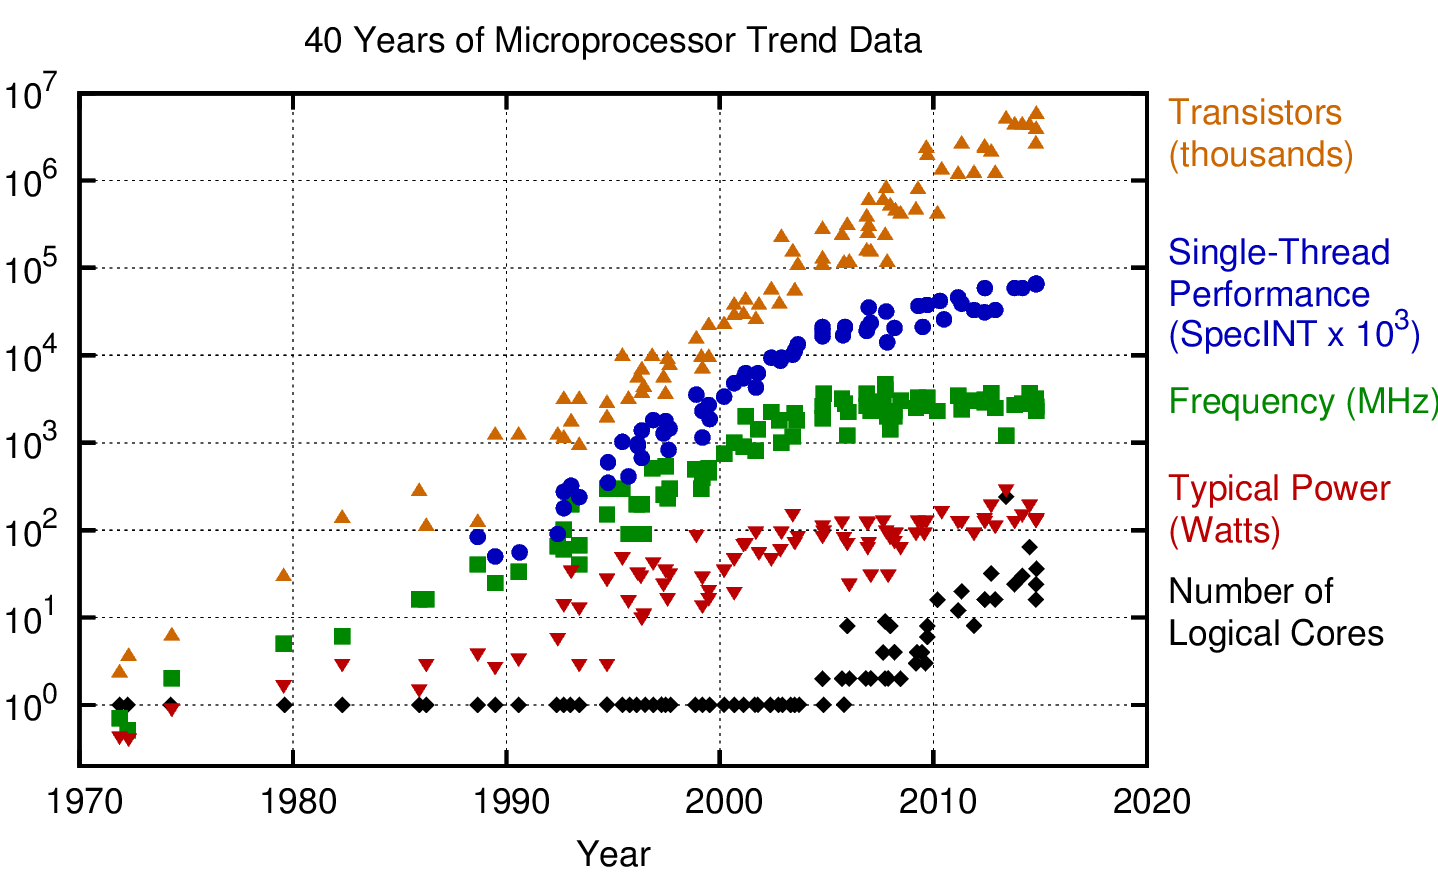
\includegraphics[width=10cm]{images/cpu_evolution.png}
    \caption{\label{pic_cpu_evolution} Évolution des caractéristiques des processeurs \cite{rupp40years}.}
\end{figure}

\begin{figure}
    \center
    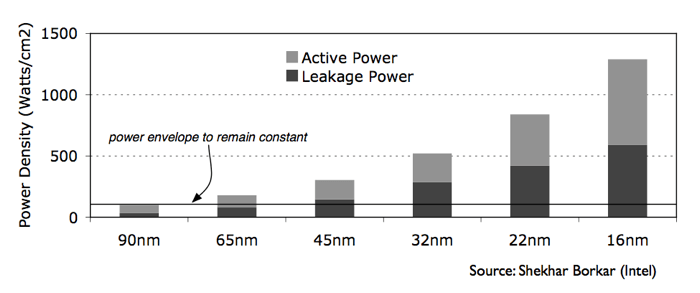
\includegraphics[width=10cm]{images/cpu_leakage.png}
    \caption{\label{pic_cpu_leakage} La miniaturisation de l'isolant nécessaire au fonctionnement des transistors permet le passage de courant de \textit{fuites}.}
\end{figure}

Bien que la fréquence des processeurs n'augmente plus depuis plus de 10 ans, la \autoref{pic_cpu_evolution} montre que la performance des processeurs continue bien d'augmenter. En effet, si la loi de Dennard n'est plus valide, la loi de Moore elle l'est encore après 2005. Les processeurs reçoivent toujours plus de transistors permettant d'augmenter la complexité des pipelines. Ces transistors sont alors utilisés pour construire des processeurs avec plusieurs coeurs. Présentés dans la \autoref{sec:multicore}, il est intéressant de remarquer que l'augmentation du nombre de coeurs commence exactement quand la fréquence n'augmente plus. Les processeurs sont alors capables de réguler la chaleur d'un processeur en plaçant les processus peu actifs sur les points chauds de la puce.
Pour limiter la consommation électrique, des techniques de management d'alimentation sont alors mises en place pour éteindre certaines parties du processeur inutilisées.
L'utilisation de différentes fréquences est aussi largement utilisée. Les processeurs possèdent des fréquences dites \textit{turbo}, leur permettant d'atteindre des fréquences très élevées pendant un court laps de temps ou lorsque le processeur n'est pas pleinement utilisé (coeurs et calculs vectoriels inutilisés).



\subsubsection{FPU}\label{sec:fpu}

Le second moyen d'accélérer l'exécution des instructions est d'utiliser des matériels spécialisés pour leur exécution. L'unité de calcul en virgule flottante (FPU pour \textit{floating-point  unit}) est un composant du processeur permettant de réaliser les opérations sur les nombres à virgule flottante. À l'origine ce module était séparé du processeur et il convenait à l'utilisateur de choisir s’il voulait ou non en brancher une sur la carte mère dans l'emplacement qui lui était alors dédié. Pour des questions de coûts d'intégration et de performance, la FPU est depuis 1989, avec la sortie du processeur Intel 80486,  intégrée au processeur. 

Au fil des années, la complexité de la FPU a augmenté. Quand elle n'était capable d'exécuter que de simples opérations à l'origine, elle peut désormais réaliser des opérations complexes (division, racine carrée, exponentielles ou des fonctions trigonométriques).  De plus, des instructions fusionnées ont fait leur apparition en 2013 dans les processeurs \textit{Haswell} de Intel et Piledriver pour AMD. Elles ont la particularité de réaliser 2 opérations en un seul cycle d'horloge du processeur. Connues sous le nom de FMA pour \textit{fused multiply-add} elles sont capables d'exécuter l'instruction $a \leftarrow b * c + d$ en un seul cycle. 

Enfin, les unités de calcul modernes sont capables d'exécuter une opération sur plusieurs données à la fois. Ce type d'instructions est dit \textit{vectoriel}. Ces instructions sont performantes pour les algorithmes qui doivent exécuter une même opération sur plusieurs données (un vecteur par exemple).
Les différentes évolutions de la FPU sont responsables de la forte augmentation de la puissance de processeur. En effet, usuellement la puissance d'un processeur est donnée par le nombre de calculs flottant qu'il peut exécuter par cycle. Le tableau \ref{tab_FPU} montre comment le nombre de FLOP par cycle évolue: pour Intel, cette performance a été multipliée par deux à chaque nouvelle version de l'architecture et les FPU modernes exécutent 8 fois plus de calculs qu'en 2008.

\begin{table}[]
\centering
\caption{Evolution de la performance des FPU}
\label{my-label}
\begin{tabular}{|l|l|l|l|l|l|}
\hline
\multicolumn{1}{|c|}{\textbf{Année}} & \multicolumn{2}{c|}{\textbf{Architecture Intel / AMD}}     & \multicolumn{1}{c|}{\textbf{Simpe p.}} & \multicolumn{1}{c|}{\textbf{Double p.}} & \multicolumn{1}{c|}{\textbf{Opérations}} \\ \hline
2008                                 & Nehalem                          & K10                     & 8                                      & 4                                       & 4 add. et 4 mul.         \\ \hline
2011                                 & Sandy Bridge                     & Bulldozer               & 16                                     & 8                                       & 8 add. et 8 mul.         \\ \hline
2013                                 & Haswell \& Skylake               &                         & 32                                     & 16                                      & 8 FMA (mult. + add.)        \\ \hline
2016                                 & Xeon Phi KNL &                         & 64                                     & 32                                      & 8 FMA (mult. + add.)        \\ \hline
\end{tabular}
\label{tab_FPU}
\end{table}

%\textbf{TODO} latence des differentes instructions; skylake FMA 4 cycles %http://agner.org/optimize/blog/read.php?i=415 (calc_fma() combien de FMA en parallele)







\subsubsection{Optimisations}
Dans les sous-parties précédentes est présenté comment l'évolution de la fréquence et l'utilisation de matériel spécialisé comme une FPU permet d'accélérer l'exécution d'une instruction. Pour différentes raisons (dépendance, manque d'un opérande), les instructions ne peuvent pas être exécutées à la vitesse maximale théorique prévue par le processeur. Pour maximiser le nombre d'instructions exécutées chaque cycle, les processeurs ont reçu de nombreuses optimisations. 

\paragraph{Exécution dans le désordre.}\label{sec:out_of_order}
 

Le but de cet optimisation est de cacher l'attente de donnée du processeur de la mémoire. Cette avancée est apparue sur les processeurs Intel en 1995 avec le \textit{Pentium P6}. Le principe de l'exécution dans le désordre est d'exécuter les instructions dans un ordre différent que celui donné par le code source.  Ainsi lorsqu'une instruction doit attendre une donnée, au lieu de perdre plusieurs cycles à attendre ces données, le processeur va exécuter les instructions qui suivent et finira d'exécuter la première quand la donnée sera chargée dans un registre. 
Cependant, ne pas exécuter le programme dans l'ordre initial peut fausser les résultats. C'est alors au processeur de s'assurer que les instructions permutées ne sont pas dépendantes. Il existe trois types de dépendances. La première est une \textit{lecture après écriture} (Read After Write ou RAW): une instruction lit une donnée écrite par une instruction la précédent. La deuxième est une \textit{écriture après lecture} (WAR): une première instruction lit une donnée qui est modifiée par une instruction la suivant. Enfin, la dernière dépendance est une \textit{écriture après écriture} (WAW): deux instructions écrivent sur la même donnée. Pour éliminer ces deux dernières dépendances, les processeurs possèdent plus de registres que ceux adressables par le programme. Il les utilise pour éliminer les dépendances WAR et WAW grâce à des techniques de renommage de registres \cite{903248}. 
L'extrait de code \ref{code_dependances} donne un exemple pour chaque type de dépendances. Dans chaque cas, la valeur de B n'est pas la même si les deux assignations ne sont pas exécutées dans le même ordre, suivant cet ordre, B peut valoir 10 ou 15. Pour ce faire, le processeur possède une fenêtre de plusieurs instructions, aussi appelée (à tord) l'\textit{execution queue}. En effet, cette liste n'a pas vocation à être exécutée dans l'ordre, c'est un rassemblement d'instructions qui ont des dépendances entre elles. Le processeur vient mettre à jour cette liste pour essayer d'exécuter des instructions qui n'ont plus de dépendances avec une donnée ou une autre instruction.
Pour pouvoir bénéficier de l'exécution dans le désordre, le processeur doit donc détecter si les instructions sont dépendantes pour pouvoir les réordonner. Aussi, le programmeur peut aider le processeur dans son travail en évitant au maximum les dépendances entre les instructions. 
La complexité apportée par le système d'exécution dans le désordre, peut être la source d'attaque comme la récente faille \textit{Meltdown} des processeurs Intel \cite{DBLP:journals/corr/abs-1801-01207}.



\begin{lstlisting}[language=C, caption=Exemples de dépendances entre deux instructions., float,floatplacement=H, label=code_dependances]
//----------- Read after Write -----------
int A, B = 0
A = 5;
B = A + 10;
//Result: B == 10 ou B == 15

//----------- Write after Read -----------
int A, B = 0
B = A + 10;
A = 5;
//Result: B == 10 ou B == 15 
 
//----------- Write after Write -----------
int B = 0
B = 10;
B = 15;
//Result: B == 10 ou B == 15
\end{lstlisting}






\paragraph{Prédiction de branchement}\label{sec:branch_predictor}
L'exécution dans le désordre fonctionne tant que suffisamment d'instructions sont disponibles pour être exécutées. Cependant, lorsqu'un programme contient un branchement conditionnel, le processeur doit attendre que sa condition soit testée. Si cette condition utilise une variable modifiée dans les instructions précédentes, le processeur doit attendre d'avoir le résultat du test pour connaître les futures instructions à exécuter. Pour maximiser l'utilisation du pipeline, le processeur peut essayer de prédire le résultat du test et ainsi continuer l'exécution. S'il s'est trompé sur la prédiction, il doit alors annuler les instructions déjà exécutées et reprendre l'exécution des autres instructions. Le temps nécessaire pour la reprise de l'exécution après une mauvaise prédiction dépend donc de la taille du \textit{pipeline} utilisé (plusieurs dizaines de cycles).
La prédiction de branchement peut être implémentée par deux méthodes.
Le processeur peut posséder un matériel spécifique, appelé prédicteur de branchement (\textit{branch predictor}), qui utilise des méthodes de statistiques. Lorsqu’un branchement est faux plusieurs fois de suite, il peut estimer qu'il y a une grande probabilité qu'il le soit aussi à l’itération suivante et éviter d’attendre le résultat du test pour continuer l’exécution. Le processeur peut aussi, à partir de l'adresse de destination, comprendre si la condition et le saut sont utilisés dans une boucle ou si c'est un retour de fonction. Une mauvaise prédiction pouvant fortement impacter l'exécution, les processeurs implémentent des prédicteurs de branchement toujours plus complexes. Ce matériel représente une part non négligeable du processeur, et des travaux ont pour objectif d'en comprendre leur fonctionnement \cite{Milenkovic2002}.
La deuxième façon d'implémenter la prédiction est réalisée statiquement, par le compilateur. À la lecture du code, le compilateur peut deviner qu'une boucle ne verra son branchement vrai qu'a la fin de son parcours. Il peut alors calculer le nombre d’itérations à réaliser et éviter le test à chaque itération.
Comme pour le mécanisme d'exécution dans le désordre, la complexité apportée par le prédicteur de branchement a donné lieu à une importante faille de sécurité découverte en 2018 par les chercheurs de Google appelée Spectre \cite{kocher2018spectre}.






%%%%%%%%%%%%%%%%%%%%%%%%%%%%%%%%%%%%%%%%%%%%%%%%%%%%%%%%%%%%%%%%%%%
\subsection{Exécuter les instructions en parallèles} \label{sec:para}
%%%%%%%%%%%%%%%%%%%%%%%%%%%%%%%%%%%%%%%%%%%%%%%%%%%%%%%%%%%%%%%%%%%

La loi de Moore a assuré aux processeurs un gain constant de transistors chaque année. Ils peuvent être utilisés pour implémenter de nouvelles fonctionnalités matérielles permettant d'exécuter les instructions en parallèle pour accélérer les applications. Les processeurs ont reçu de nombreuses améliorations dont les principales sont présentées dans cette section: 
\begin{itemize}
    \item Le pipeline
    \item Les processeurs superscalaire
    \item Les coeurs
\end{itemize}


\subsubsection{Le pipeline} \label{sec:pipeline}
%%%%%%%%%%%%%%%%%%%%%%


\paragraph{Motivations.} 

L'utilisation d'instructions CISC toujours plus complexes a pour effet d'allonger le temps nécessaire à leur exécution qui dure alors plusieurs cycles. Les instructions complexes nécessitent plusieurs opérations: le chargement, depuis la mémoire (\textit{fetch}), le décodage (\textit{decode}), le chargement des données nécessaires (\textit{memory}), l'exécution (\textit{execute}) et l'enregistrement du résultat (\textit{write-back}). Pendant ces différentes étapes, la totalité de l'unité d'exécution n'est pas disponible pour les instructions suivantes. 

La chaîne de traitement du processeur, ou \textit{pipeline}, est une implémentation matérielle d'un module qui permet de découper l'exécution d'une instruction en plusieurs étapes (\autoref{pic_pipeline_simple}). Cette technique peut être vu pas analogue à l'utilisation de chaîne de montage. Datant de plus d'un siècle, la technique de la chaîne de montage a été abondamment utilisée par des industriels tels que Louis Renault et Henry Ford \cite{wolff1957entrepreneurs}.



\begin{figure}
    \center
    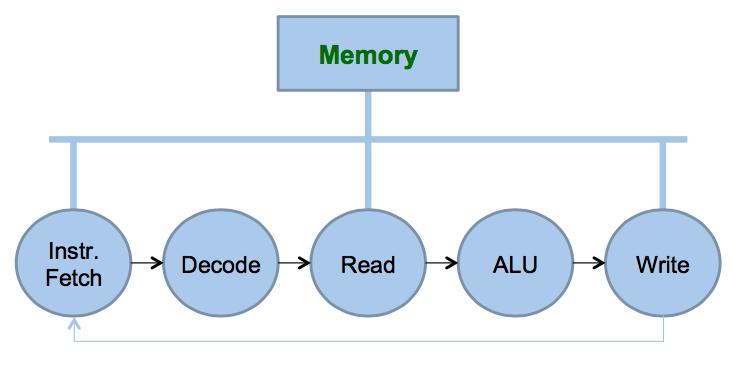
\includegraphics[width=10cm]{images/Chapitre1/Neumann.png}
    \caption{\label{pic_pipeline_simple} Représentation simplifié d'un pipeline de 5 étapes.}
\end{figure}


\paragraph{Implémentation}

En informatique, la technique de \textit{pipeline} est utilisée pour exploiter le parallélisme d'instructions (ILP) (\autoref{pic_pipeline}). Il est commun de présenter la notion de pipeline avec un pipeline de 5 niveaux:

\begin{itemize}
    \item \textbf{Recherche de l'instruction} ou \textit{fetch}: cette première étape charge l'instruction à exécuter depuis la mémoire principale dans un registre du processeur. Grâce à un compteur interne, le registre \textit{Program Counter}, le processeur connaît l'adresse mémoire de la prochaine instruction à charger. Pour améliorer le temps d'accès aux instructions, le processeur possède un tampon (\textit{instruction buffer}) contenant plusieurs instructions d'avance.
    \item \textbf{Décodage} ou \textit{décode}: une fois que l'instruction est chargée, elle est décodée pour déterminer l'action à exécuter et les données nécessaires.
    \item \textbf{Execution} ou \textit{execute}: en fonction du décodage réalisé, l'instruction est exécutée: utiliser l'ALU pour faire une opération ou calculer une adresse.
    \item \textbf{Accès mémoire} ou \textit{memory}: réalise un accès mémoire (\textit{load} ou \textit{store}) lorsqu'une instruction le nécessite.
    \item \textbf{Ecriture du résultat} ou \textit{write back}: enfin le processeur doit enregistrer le résultat produit par l'étape \textit{execute}. Si c'est un branchement, il modifie le registre \textit{Program Counter} (\textit{branch}). Si c'est une opération arithmétique, il sauvegarde le résultat dans l'adresse destinataire décodé par la deuxième étape.
\end{itemize}

Le fait de partager l'exécution d'une instruction en sous-étapes permet de commencer l'exécution de la suivante pendant que l'instruction actuelle est encore dans la chaîne d'exécution (voir \autoref{pic_pipeline}). Son utilisation ne réduit pas le temps d'exécution d'une instruction (5 cycles sur la \autoref{pic_pip_no}). Celles-ci doivent tout de même passer une à une par chaque étape de la chaîne. Le \textit{pipeline} permet d'améliorer la cadence d'exécution en maximisant l'utilisation de chaque ressource à un même moment (\autoref{pic_pip_yes}). On peut par exemple commencer à charger la prochaine instruction (étape \textit{fetch}), alors que l'instruction actuelle est en train d'être exécutée (étape \textit{execute}). Sur la \autoref{pic_pip_yes} on assiste à l'exécution de 5 instructions, au premier temps une seule instruction est exécutée, à l'étape $IF$ pour \textit{instruction fetch}. Ensuite, une nouvelle instruction est chargée (opération $IF$) pendant que la première est passée à l'étape suivante (opération $ID$). Ainsi au bout de 5 cycles, chaque étape du pipeline est utilisée (partie en verte). 


\begin{figure}
    \begin{subfigure}[]{0.5\linewidth}\centering
        \vspace{1.6cm}
        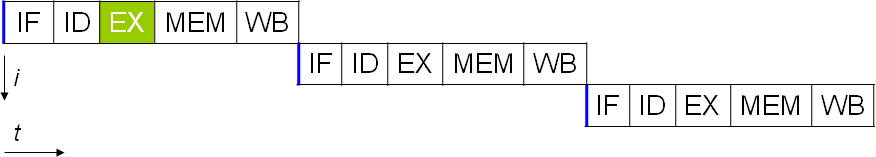
\includegraphics[width=\linewidth]{images/Chapitre1/pipelineNo.png}
        \caption{Processeur sans pipeline \label{pic_pip_no}}
    \end{subfigure}%
    ~ %space
    \begin{subfigure}[]{0.5\linewidth}\centering
        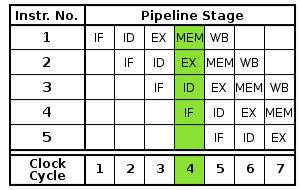
\includegraphics[width=.7\linewidth]{images/Chapitre1/pipelineYes.png}
        \caption{Processeur avec un pipeline à 5 étages \label{pic_pip_yes}}
    \end{subfigure}
    
    \caption{Pipeline: en séquençant les instructions, le processeur est capable d'exécuter des étapes différentes en parallèle (\textit{IF: instruction fetch, ID: instruction decode, EX: execution, MEM: memory, WB: write back}). Le nombre de cycles nécessaires pour l'exécution de 3 instructions passe alors de 15 à 8 cycles (source: \url{https://fr.wikipedia.org/wiki/Pipeline_(architecture_des_processeurs)} }
    \label{pic_pipeline}
\end{figure}




\paragraph{Taille du pipeline.}
En 1939 IBM conçoit le premier processeur avec pipeline. Ce n'est qu'en 1989 qu'Intel produira le sien (Intel 80486). Le nombre d'étapes (ou profondeur du pipeline) était de deux à l'origine. Cette taille a augmenté au fil du temps atteignant 31 étapes pour l'architecture du Pentium 4 Prescott d'Intel en 2004. 

\paragraph{Complexité de la gestion du pipeline.}
L'utilisation d'un \textit{pipeline} n'est pas toujours optimale et plusieurs facteurs peuvent affecter sa performance. Le principe du pipeline repose sur le concept de commencer à exécuter des instructions avant que la précédente ne soit terminée. Cela peut être rendu impossible par la dépendance entre deux instructions et par l'utilisation de branchements conditionnels \cite{emma1987characterization}. Lors de l'évaluation d'un tel branchement, le pipeline ne peut pas commencer à exécuter les instructions suivantes sans connaître son résultat. Le processeur doit alors attendre (\textit{stall}) plusieurs cycles avant de continuer. Une optimisation de prédiction de branchement a été implémentée pour éviter ces états de \textit{stall} (voir \autoref{sec:branch_predictor}). De plus, pour permettre la bonne utilisation du pipeline, des mémoires tampons doivent être disposées entre chaque étape pour mémoriser les différents résultats intermédiaires. Lorsque le processeur exécute plusieurs processus, il doit veiller à terminer l'exécution des instructions avant de commencer celles du processus suivant. La complexité de sa gestion le rend vulnérable aux attaques informatiques (voir \autoref{sec:out_of_order}). 













\subsubsection{Processeur superscalaire} \label{sec:superscalar}
%%%%%%%%%%%%%%%%%%%%%%

Le pipeline apporte un niveau de parallélisation horizontale. Les processeurs ont reçu une autre amélioration apportant au pipeline une parallélisation verticale. 

\paragraph{Principe}
Un processeur est dit \textit{superscalaire} s'il est capable d'exécuter plus d'une instruction simultanément. Le nombre d'instructions par cycle d'horlge (IPC) peut alors être supérieur à 1. Le principe est d'implémenter un second pipeline (ou plus) capable d'exécuter les instructions telles que sur la \autoref{pic_pip_yes}. Intel proposa son premier processeur superscalaire en 1989 avec le processeur Intel 80486. Il possédait un pipeline à cinq étages proche de celui présenté dans la section précédente. 
Pour pouvoir l'utiliser, le processeur doit déterminer si deux instructions peuvent être exécutées en parallèle (sans dépendance et utilisant des ressources matérielles différentes). La \autoref{pic_superscalar} montre comment une implémentation superscalaire du pipeline fonctionne. 

\begin{figure}
    \center
    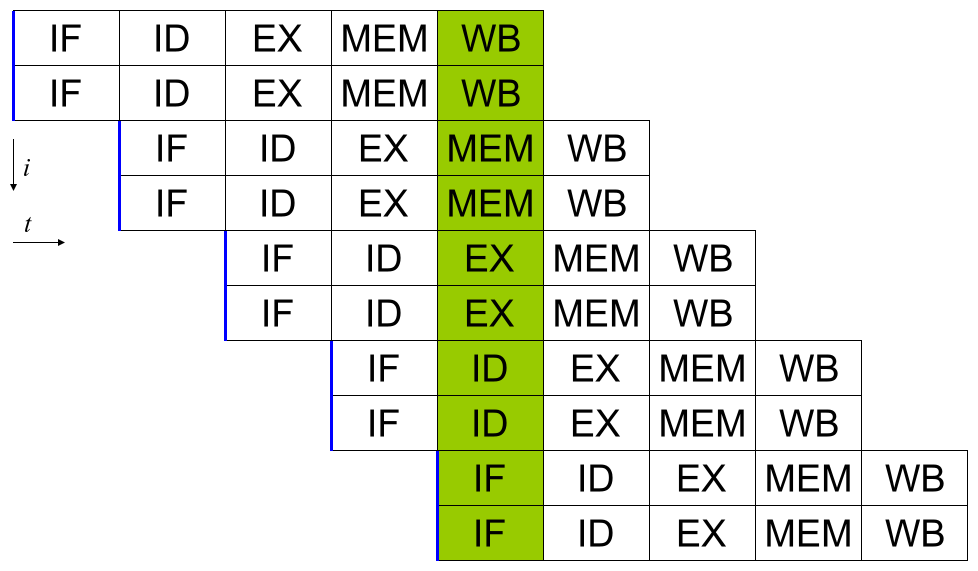
\includegraphics[width=8cm]{images/Chapitre1/superscalar.png}
    \caption[Processeur superscalaire]{Fonctionnement d'un processeur superscalaire possédant deux pipelines.\protect\footnotemark. \label{pic_superscalar} }
\end{figure}
\footnotetext{source: \url{https://fr.wikipedia.org/wiki/Processeur_superscalaire}}

\paragraph{Implémentation}
Il existe deux façons de transformer un processeur scalaire en superscalaire. La première est de dupliquer matériellement chaque étape pour obtenir deux pipelines distincts (processeurs \textit{superpipeline}). On peut citer le processeur Intel Pentium dont la totalité du pipeline n'est pas dupliquée. Le processeur à une fenêtre de plusieurs instructions prêtes à être exécutées. Seule la phase d'exécution est dupliquée.  Il possédait deux unités d'exécution \textit{u} et \textit{v} qui pouvait exécuter des instructions de types différents (opérations flottantes ou entières) en parallèle. 
Le deuxième moyen d'implémenter le parallélisme d'instruction d'un processeur superscalaire repose sur le fait qu'une étape peut nécessiter moins d'un demi-cycle d'horloge pour être exécutée. Une étape (ou micro-instruction) du pipeline peut donc s'occuper de deux instructions différentes pendant un cycle d'horloge, en utilisant sa propre horloge interne. Cette méthode a le bénéfice de ne pas avoir a dupliquer le pipeline matériellement. 

Les principales limitations à l'implémentation d'un pipeline sont les dépendances et les conflits. Cela peut être une dépendance entre les données de plusieurs instructions ou un conflit d'accès à une même ressource (ALU, FPU). Le processeur est alors en charge d'orchestrer les différentes instructions pour rendre possible le parallélisme en utilisant des stratégies \textit{d’émission} \cite{johnson1989super} des instructions. Cette stratégie doit veiller à conserver la validité du programme en veillant aux ordres: de lecture des instructions, de leur exécution et de leur actualisation des registres (ou de la mémoire). 


\paragraph{Exemple du Pentium 4}\autoref{sec:alu_pentium}
Pour bien comprendre le déroulement de l'exécution du pipeline d'un processeur superscalaire, nous choisissons de détailler le fonctionnement de processeur Intel Pentium 4 \cite{stallings2003organisation} donc le schéma de la microarchitecture est présenté sur la \autoref{cpu_superscalar_pentium}. Le processeur exécute les \textit{micro-ops} en utilisant un pipeline d'au moins 20 étages en veillant à respecter les dépendances, dont les principales étapes sont décrites ici: 

\begin{enumerate}     
\item Le processeur lit les instructions (CISC) depuis le cache L2 par groupe de 64 octets dans l'ordre du programme pour profiter de l'effet de localité. Bien que la prédiction de branchement puisse modifier cet ordre. 
\item Chaque instruction (pouvant être de taille différente) est décodée et traduite en une à quatre instructions RISC de 118 bits (\textit{micro-ops}). 
\item Ces micro-ops sont ensuite stockés dans un buffer (\textit{Trace Cache}) permettant l'utilisation de l'exécution dans le désordre (voir \autoref{sec:out_of_order}).
\item Ensuite, le processeur procède au renommage des registres. Il existe 16 registres architecturaux (utilisable par le code) mais 128 registres physiques sont réellement implémentés. Les \textit{micro-ops} peuvent ensuite être stockée dans deux listes d'attente distinctes utilisant une discipline \textit{FIFO}.
\item L'ordonnanceur choisi ensuite dans les deux files les instructions qui possèdent leurs opérandes et dont l'exécution peut être réalisée. Suivant le type d'instruction, elles sont envoyées (jusqu'à 6 à la fois) vers l'unité d'exécution correspondante (calcul entier ou flottant) en utilisant les différents ports. 
\end{enumerate}
     

\begin{figure}
    \center
    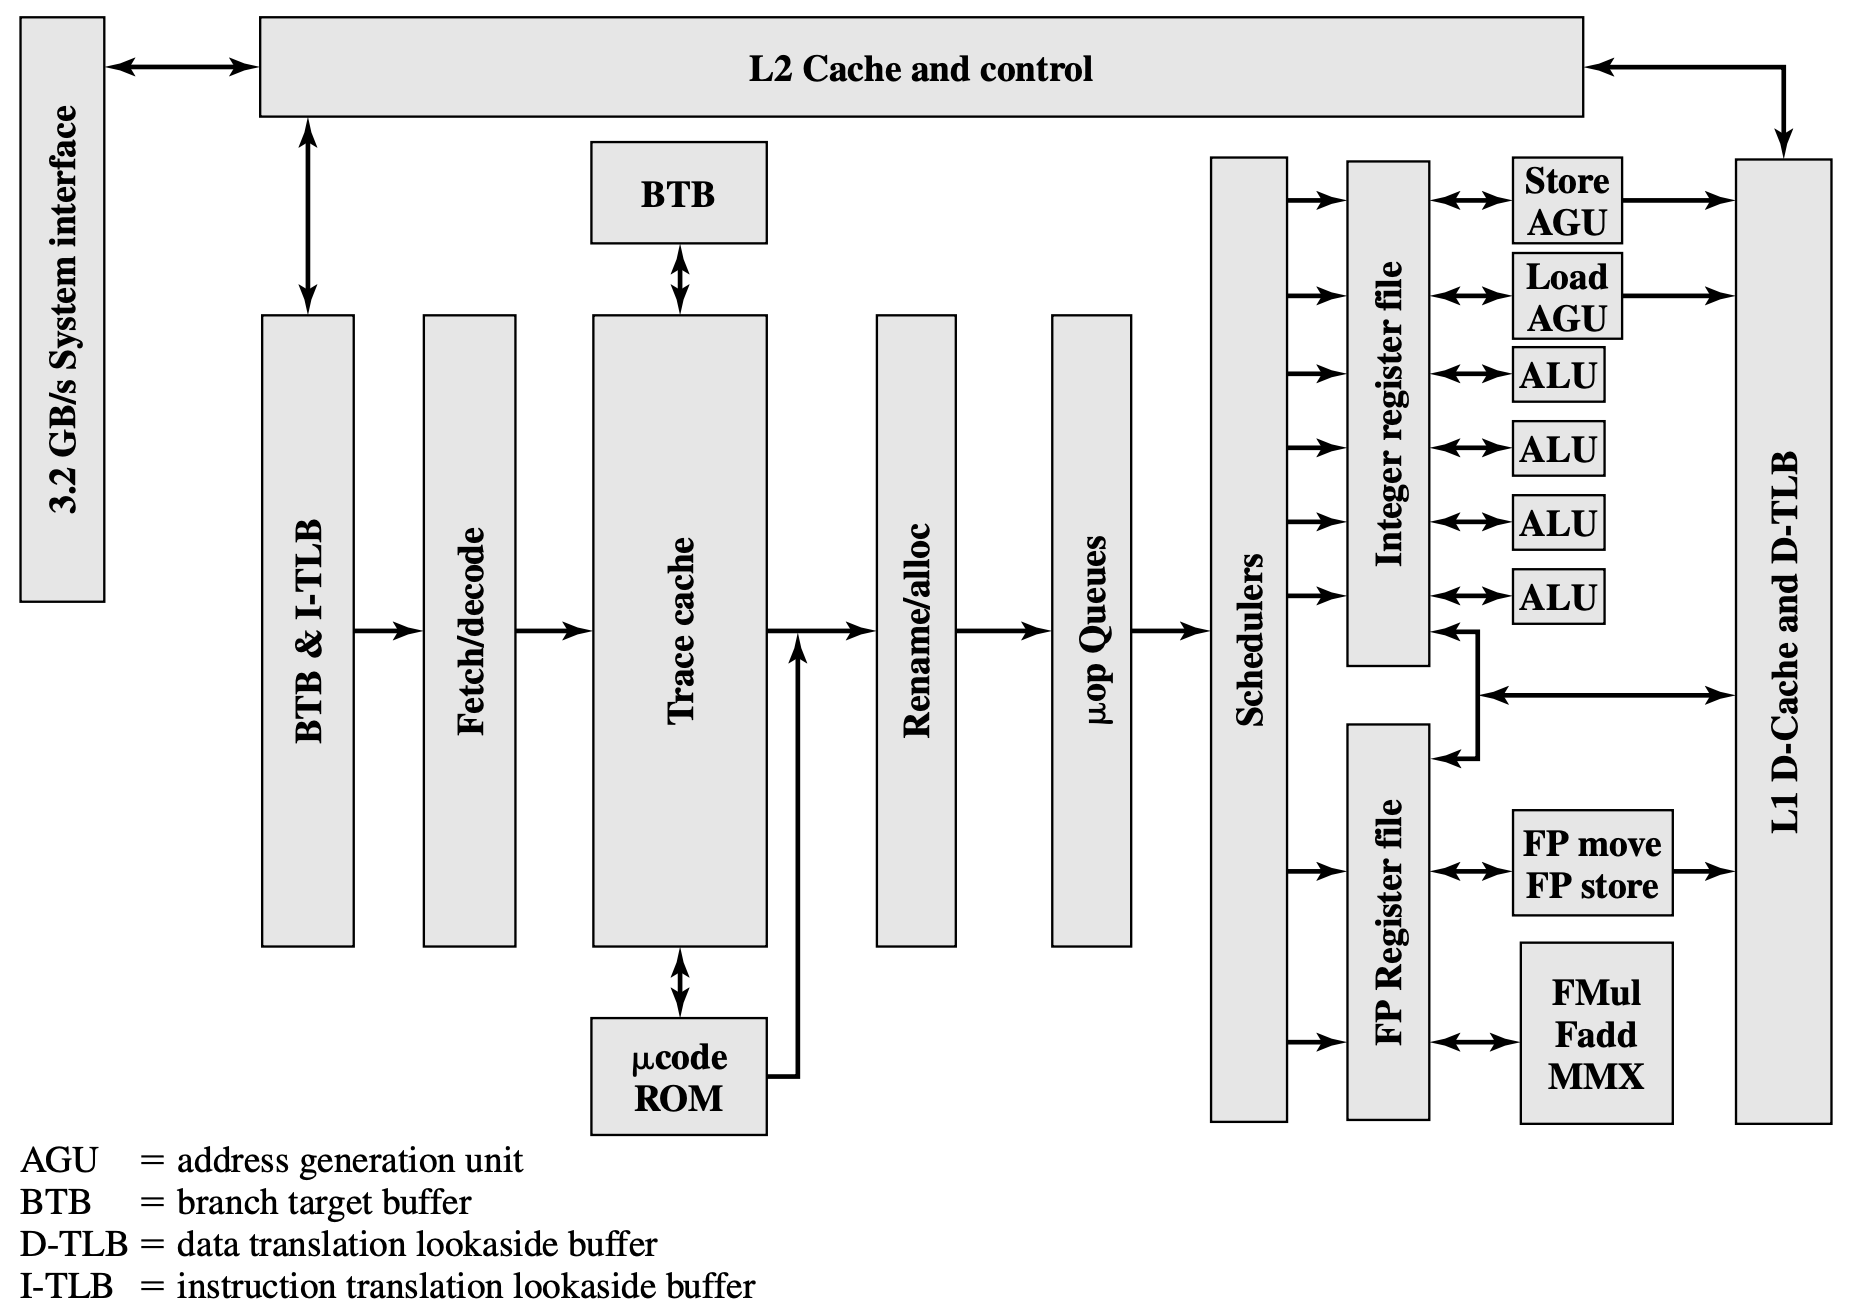
\includegraphics[width=13cm]{images/cpu_superscalar_pentium.png}
    \caption[Diagramme en bloc du Pentium 4]{Diagramme en bloc du Pentium 4 \cite{stallings2003organisation}
    \label{cpu_superscalar_pentium}}
\end{figure}



Les architectures actuelles ont beaucoup évolué depuis le premier pentium. Le détail de la microarchitecture Skylake d'Intel peut être consultée dans l'annexe \autoref{pic_cpu_skylake_architecture}. L'unité d'exécution peut être utilisée par 8 \textit{ports} différents. Chaque port est relié à des composants différents de l'ALU qui peut exécuter jusqu'à 4 instructions par cycles (ou 2 opérations flottantes).






\subsubsection{Processeur multi-coeurs} \label{sec:multicore}
%%%%%%%%%%%%%%%%%%%%%%


\paragraph{Motivation.}
La vitesse de calcul d'un processeur est liée à sa fréquence qui a largement contribué à l'évolution de leur performance. Cependant, certaines limites physiques empêchent l'augmentation infinie des fréquences (discuté dans la partie \ref{sec:frequency}). Il a donc fallu trouver d'autres moyens d'améliorer la performance des processeurs, sans pouvoir accélérer leur fréquence. L'apparition des processeurs multi-coeurs est une réponse à ce challenge. Pour comprendre leur intérêt l'analogie suivante peut être utilisée \cite{tanenbaum2016structured}: la construction d'un processeur avec une fréquence de 1000 GHz est probablement impossible. Par contre, l'utilisation de 1000 processeurs avec une fréquence de 1 Ghz est possible pour obtenir la même performance. Ce gain de performance peut alors être utilisé pour réduire la fréquence des processeurs. En réduisant la fréquence de 30\%, l'énergie nécessaire est réduite de 35\% \cite{mattsson2014haven}. En utilisant deux coeurs à 70\% de la fréquence initiale permet cependant d'obtenir un gain de 140\% de la puissance de calcul totale. C'est ce constat qui motive l'utilisation du parallélisme dans toute l'architecture d'un supercalculateur (voir \autoref{sec:parallelisme}). Ainsi, avant l'apparition des processeurs multicoeurs, l'utilisation du multitraitement symétrique (SMP) utilisant plusieurs processeurs en parallèle était le principal moyen d'accéder au parallélisme. Cependant, les serveurs devenant toujours plus gros, et avec le désir d'avoir des processeurs plus puissant pour les ordinateurs personnels et les téléphones, les processeurs multi-coeurs ont été inventés.


\paragraph{Multi-coeur.}
Le terme de processeur multi-coeur est employé pour désigner tout processeur possédant entre deux et quelques dizaines de coeurs (on parle de processeurs \textit{manycore} au-delà). Les différents coeurs sont disposés sur la même puce d'où l'autre appellation utilisée pour désigner ces processeurs de Chip Multiprocessor (CMP).
Les différents coeurs sont généralement identiques en tout point (processeur homogène) bien qu'ils puissent être différents (processeur hétérogène). Les processeurs homogènes sont plus faciles à utiliser, car tous les coeurs peuvent répondre au même besoin et leur design est plus simple. Les processeurs hétérogènes sont cependant plus performants pour certaines applications. 
Généralement, chaque coeur du processeur n'est pas relié directement à la mémoire. Un niveau de cache est généralement interposé entre le coeur et la mémoire. La hiérarchie mémoire est présentée dans la \autoref{sec:hierarchie}.

\begin{figure}
    \center
    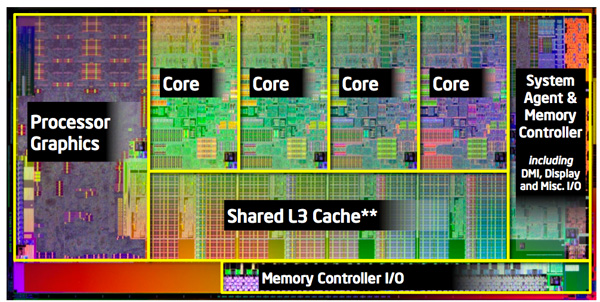
\includegraphics[width=10cm]{images/cpu_multicore.jpg}
    \caption{\label{processeur_archi} Exemple de processeur multi-coeur (Intel Core i7-2600K)  partageant le troisième niveau de cache.\protect\footnotemark}
\end{figure}

\footnotetext{source: \url{https://www.anandtech.com/show/4083/the-sandy-bridge-review-intel-core-i7-2600k-i5-2500k-core-i3-2100-tested}}



L’avantage principal de dupliquer un coeur plutôt que de doubler la fréquence d’un seul coeur est la consommation électrique et donc la puissance dégagée par effet Joule. En effet, la puissance dissipée est quadruplée quand la fréquence est doublée alors qu'elle ne fait que doubler lorsque le nombre de coeurs est doublé. On obtient ainsi un processeur utilisant moins d’énergie et nécessitant moins de refroidissement pour une même performance qu'un processeur plus rapide.
Comme pour le pipeline (voir \autoref{sec:pipeline}), le gain de performance apporté par l’ajout de coeur s’appuie sur l’amélioration du parallélisme d'instruction (Instruction Level Parallélisme (ILP)).


La difficulté d’utilisation de processeurs multi-coeurs vient des programmes qui ne sont pas capables par nature d’utiliser ce niveau de parallélisme. Ils doivent donc être programmés pour pouvoir en profiter. Cette tâche, quoique difficile à ses débuts, est aujourd'hui facilitée par l’utilisation de librairies prévues telles que \textit{Pthread} ou \textit{OpenMP}. 

Les coeurs partagent des niveaux communs de cache (généralement le dernier), la bonne programmation des applications et l'implémentation d'une microarchitecture efficace sont alors des facteurs déterminants de la performance obtenue:
\begin{itemize}
    \item Pour maximiser l'utilisation des caches, il est primordial de prévoir leurs partages entre les différents coeurs pour minimiser les conflits. Des méthodes de placements plus ou moins efficaces peuvent alors être utilisées \cite{mazouz2011performance}: laisser le système d'exploitation s'en occuper peut donner des performances très variables entre deux exécutions identiques, alors que le placement manuel permet d'obtenir les meilleurs résultats. 
    \item Le choix du réseau utilisé par les coeurs est alors important pour la performance des codes et repose principalement sur quatre paramètres \cite{peh2009chip} : la topologie, les algorithmes de routages, le protocole de contrôle de flux et le routage de la microarchitecture. La topologie indique comment les coeurs sont connectés et quels sont les chemins empruntables par un message pour rejoindre sa destination. Ce choix est réalisé par l’algorithme de routage. Le contrôle de flux s’occupe de l'envoi des messages (ordre et date d’envoi) qui est ensuite réalisé par la microarchitecture. Les choix réalisés pour ces quatre paramètres ont un impact sur la performance du processeur (latence, bande passante) et sur son prix. 

\end{itemize}

Le nombre de coeurs par processeur a beaucoup évolué dans les quinze dernières années. Si les premiers processeurs multi-coeurs n'en possédaient que deux, il n'est pas rare que les supercalculateurs utilisent des processeurs avec plus de vingt coeurs. Intel à même annoncé en 2019 un nouveau processeur doté de 56 coeurs \footnote{\url{https://ark.intel.com/content/www/us/en/ark/products/194146/intel-xeon-platinum-9282-processor-77m-cache-2-60-ghz.html}}. Cependant, l'ajout de coeurs supplémentaires n'est pas forcément bénéfique pour les applications à cause de la vitesse des mémoires qui peinent à évoluer au même rythme. Ce constat est discuté dans la \autoref{sec:memory}.
